\documentclass[12pt]{article}
\usepackage[margin=1in]{geometry}
\usepackage{graphicx}
\usepackage{booktabs}
\usepackage{array}
\usepackage{xcolor}
\usepackage[hidelinks]{hyperref}
\usepackage{authblk}
\usepackage{caption}
\captionsetup{font=small,labelfont=bf}
\setlength{\parskip}{0.55em}
\renewcommand{\baselinestretch}{1.07}
\newcommand{\boxnote}[1]{\begin{center}\fbox{\begin{minipage}{0.93\linewidth}#1\end{minipage}}\end{center}}
\newcolumntype{P}{>{\centering\arraybackslash}p{2.2cm}}

\title{\textbf{Teaching an AI to Double-Check Its Own Work}\\[3pt]
\large Review Residuals --- an illustrated, plain-English companion}
\author[ ]{Kyle Kramer}
\affil[ ]{NeraTech LLC}
\date{June 2026}

\begin{document}
\maketitle

\boxnote{\textbf{In one sentence.} Today's AI models accept every internal step blindly; we added a small
``check it before you commit to it'' step---borrowed from how pilots, surgeons, and nuclear operators avoid
mistakes---and found that it does nothing for small models but, as the models grow, starts to win, until at the
largest sizes we tested it beats the standard method today's AI actually uses.}

This companion walks through the same idea, figures, and results as our technical paper, but in everyday
language. Every figure and table from the research version is here, each with a plain explanation of what it
shows and why it matters.

\section*{1.\quad What kind of AI are we talking about?}
The AI behind tools like ChatGPT is a \emph{language model}. At its core it does one simple thing: read some
text and predict what comes next, one piece at a time. To do that well it passes the text through many stacked
\emph{layers}, each refining the model's internal sense of things before handing it on. Picture a long assembly
line: a sentence goes in one end, passes through dozens of stations, and a polished prediction comes out the
other.

\section*{2.\quad The hidden problem: the AI trusts every step blindly}
At every station on that assembly line, the layer \emph{proposes a change} to the work-in-progress---and that
change is \textbf{applied automatically, in full, every time}. There is no inspection step. Nothing pauses to
ask, ``is this particular change actually a good idea?'' Some changes are great, some are noise; the machine
trusts them all equally. It works remarkably well anyway---but it's a strange way to build something this
important. (The technical name for the wiring that does this is a ``residual connection''; the plain version is:
every step is accepted, no questions asked.)

\section*{3.\quad The fix comes from aviation, surgery, and nuclear power}
Those fields solved this exact problem long ago---and the reason they had to is worth sitting with. Even
brilliant, fully-attentive experts miss things. In a famous experiment, people asked to count basketball passes
completely failed to notice a person in a gorilla suit stroll through the middle of the scene~\cite{simons1999}.
The lesson isn't that those people were dim; it's that \emph{every} mind, human or machine, has hard limits on
what it can attend to and get right---intelligence itself is \emph{bounded}, and you can't fix that by demanding
more of it~\cite{kramer2026}. So high-reliability fields engineer checks \emph{around} the expert, and they even
have a name for the toolkit: \emph{human-performance (HP) tools}. Pilots read a step back before doing it
(self-checking); a second person confirms critical actions (peer-checking); and, most relevant here, a proposed
action is checked before it is committed---\emph{independent verification}~\cite{doe2009}. A simple pre-surgery
checklist built on these ideas measurably cut deaths. The common thread is never ``hire smarter people''---it is
\emph{build a check into the process itself}. We asked: what if we built one of those HP tools---independent
verification---into the AI?

\section*{4.\quad Our idea: a built-in ``trust dial''}
Before each layer's proposed change is applied, we add a small learned \emph{trust dial}. It looks at two
things---where the work stands now, \emph{and} the specific change being proposed---and decides how much of that
change to let through. That second part is what's new.

\begin{figure}[h]
\centering
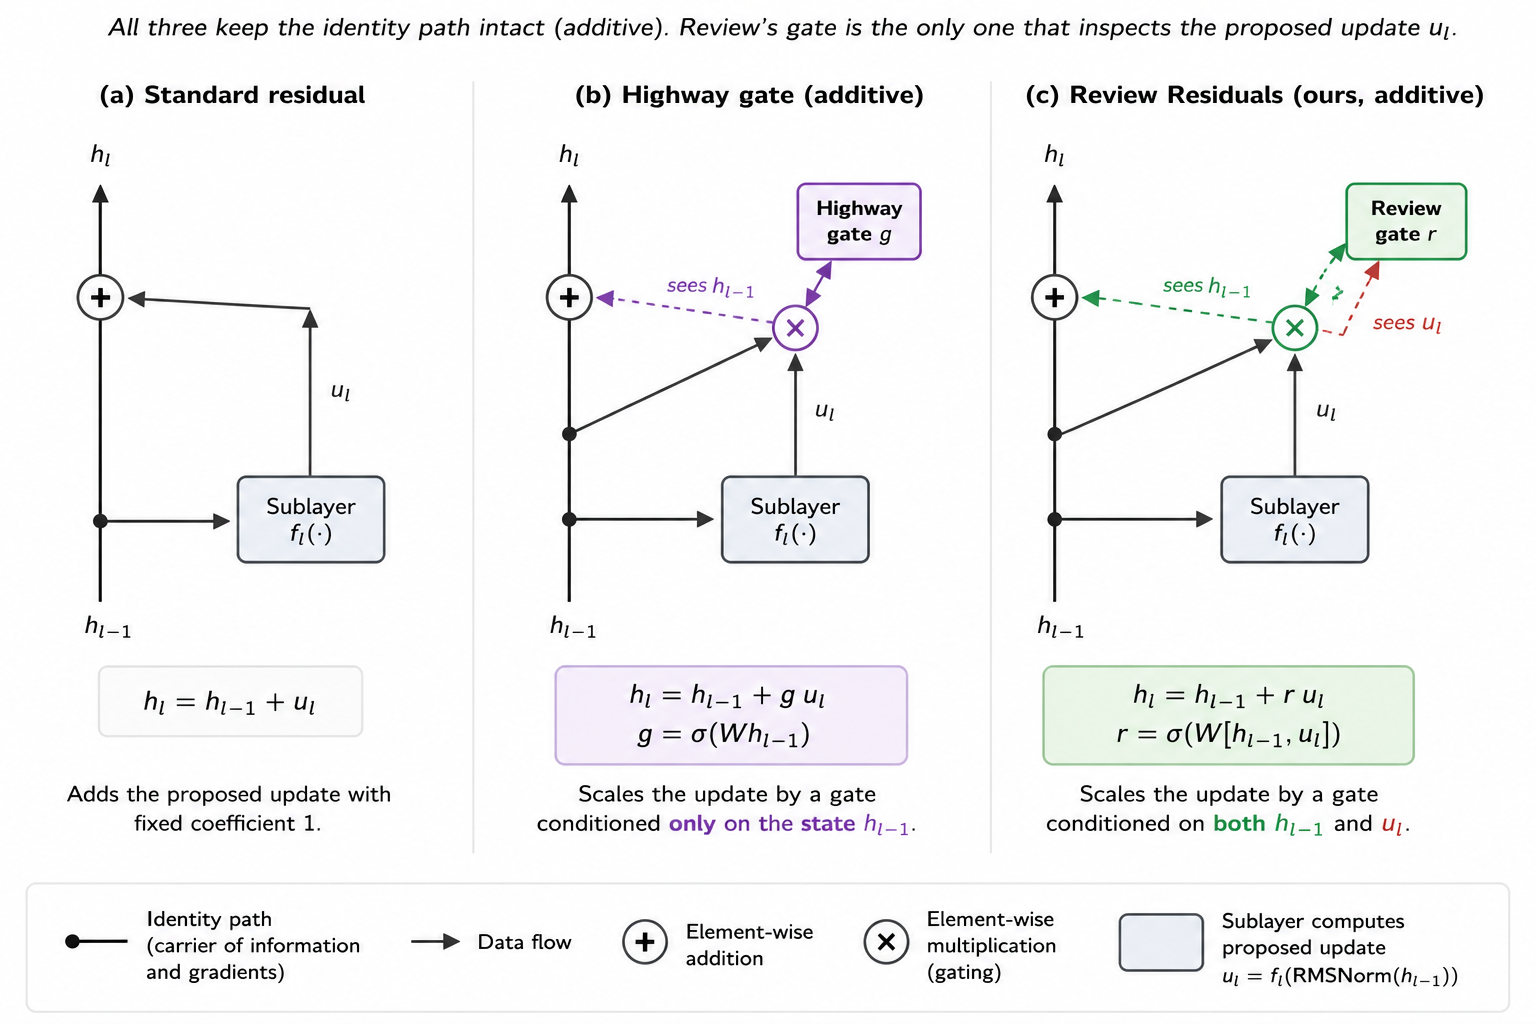
\includegraphics[width=\linewidth]{mechanism_additive.png}
\caption{\textbf{(Figure 1 from the paper.)} Three ways to handle a proposed change, all keeping the original
work intact. (a)~Standard: accept the change fully, always. (b)~Highway, the closest existing method: a dial
that looks only at the current situation. (c)~Review Residuals (ours): a dial that looks at both the situation
\emph{and} the specific proposed change (the red arrow).}
\label{fig:mech}
\end{figure}

\noindent\textbf{How to read Figure~\ref{fig:mech}:} in all three pictures the vertical line is the
``work so far,'' flowing upward untouched. The box on the right is the layer proposing a change. The difference
is the dial: the standard approach has none (it adds the whole change); Highway's dial peeks only at the work
so far; ours (the red arrow) is the only one that actually \emph{looks at the proposed change itself} before
deciding how much to trust it---like an inspector who picks up the part and examines it, rather than just
glancing at the line.

\section*{5.\quad How our idea compares to the others}
Researchers have tried several ways to control how much of each step to apply. Table~\ref{tab:pos} lays them
out. Only the last column matters for what's new here.

\begin{table}[h]
\centering
\small
\begin{tabular}{@{}p{4.4cm}p{3.8cm}PP@{}}
\toprule
\textbf{Method} & \textbf{What it adjusts} & \textbf{Reacts to the input?} & \textbf{Looks at the proposed change?}\\
\midrule
Standard (what AI uses today) & nothing --- adds it all & no & no\\
ReZero / Fixup / LayerScale & a fixed ``volume knob'' & no & no\\
Highway~\cite{srivastava2015} & a dial set by the situation & yes & no\\
Attention Residuals~\cite{kimi2026} & blends across many steps & yes & not directly\\
\textbf{Review Residuals (ours)} & a dial set by situation \emph{and} change & yes & \textbf{yes}\\
\bottomrule
\end{tabular}
\caption{\textbf{(Table 1 from the paper, in plain terms.)} Every prior method either ignores the input or
reacts only to the current situation. Ours is the only one that looks at the \emph{specific change being
proposed} before deciding how much of it to apply.}
\label{tab:pos}
\end{table}

\section*{6.\quad A wall we hit---and climbed}
This part shows the work was done carefully. Our first version of the dial used a particular bit of math that
worked fine for small models but, at large sizes, \textbf{would not train at all}---the model got stuck and
learned almost nothing. We diagnosed exactly why (the math was starving the deepest layers of the learning
signal they need---the same problem a famous 2015 breakthrough was invented to fix~\cite{he2016}) and corrected it with a
principled change that keeps the original work flowing through untouched. After the fix, the large models
trained cleanly. Finding and fixing that wall is itself a useful result.

\section*{7.\quad How we tested it (a fair race)}
An AI model starts knowing nothing; we show it a big pile of text and have it practice predicting the next
piece, adjusting itself millions of times. To score it, we test on text it has never seen and measure how
\emph{surprised} it is---less surprise is better, so throughout, \textbf{lower numbers are better}. We built
the competing methods too and trained them all under identical conditions, ran each several times from
different starting points to rule out luck, and---crucially---gave the competitors \emph{extra size} so they
had at least as many ``parts'' as ours. That last point matters: it means any win can't just be because our
method is bigger.

\section*{8.\quad What we found}
We trained five sizes, from small up to one billion parameters. Table~\ref{tab:res} has the actual scores, and
Figure~\ref{fig:scale} shows the pattern.

\begin{table}[h]
\centering
\small
\begin{tabular}{@{}lcccc@{}}
\toprule
\textbf{Model size} & \textbf{Ours (Review)} & \textbf{Highway} & \textbf{Standard} & \textbf{Did ours win?}\\
\midrule
60M (small)      & 1.6891 & 1.6923 & \textbf{1.6805} & no --- standard was better\\
150M             & 1.5576 & 1.5625 & 1.5548 & tie\\
320M             & \textbf{1.5001} & 1.5042 & 1.5037 & tie (barely ahead)\\
590M             & \textbf{1.4795} & 1.4889 & 1.4901 & \textbf{yes, clearly} (statistically solid)\\
1B (largest)     & \textbf{1.4876} & 1.5031 & 1.5040 & \textbf{yes, by more} (strong trend)\\
\bottomrule
\end{tabular}
\caption{\textbf{(Table 2 from the paper, in plain terms.)} Scores are ``surprise'' --- lower is better. Read
top to bottom and watch it change: at the smallest size the plain standard method actually beats ours; through
the middle it's a tie; then at the two largest sizes ours pulls clearly ahead of \emph{both} the alternative
and the standard method.}
\label{tab:res}
\end{table}

\begin{figure}[h]
\centering
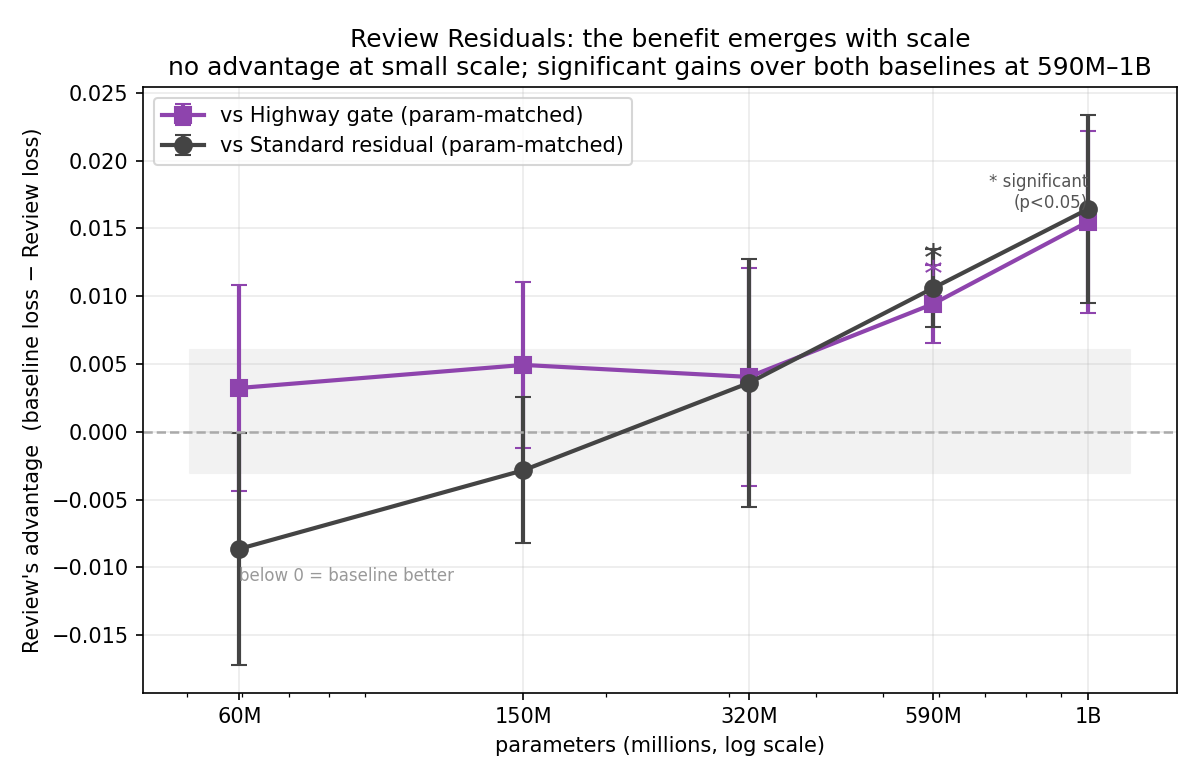
\includegraphics[width=0.80\linewidth]{emergence_curve.png}
\caption{\textbf{(Figure 2 from the paper.)} How far ahead our method is, as the model grows (left to right).
Above the dashed line = ours is better; below = the other method is better. Both lines start at or below the
line for small models and rise clearly at the largest sizes. The star marks where the win is statistically
solid.}
\label{fig:scale}
\end{figure}

\noindent\textbf{How to read Figure~\ref{fig:scale}:} the horizontal axis is model size (small on the left, a
billion on the right). The vertical axis is how much better our method is---above the dashed line we win, below
it the other method wins. The grey line (versus the plain standard method) literally \emph{starts below the
line}---the standard beats us on small models---then climbs and ends well above it at a billion parameters. The
purple line (versus the alternative dial) does the same. In plain terms: \textbf{the benefit emerges as the
models get bigger}. That's unusual and encouraging---most clever tweaks get \emph{harder} to justify as models
grow; this one got \emph{easier}.

\section*{9.\quad What's encouraging --- and what we're not claiming}
\textbf{What's encouraging is real.} This is a fresh idea, drawn from a safety tradition almost nobody has
applied to AI. At the largest scale we could test, it beats the \emph{standard} method---not just an
alternative---and the advantage grows with size.

\textbf{And what to keep in perspective.} These are still small models by industry standards, the winning
margin is about one percent, the billion-parameter result is a strong trend that points the same way as the clear win just below it, and
we tested on one simple kind of text~\cite{eldan2023}. None of that is a strike against the idea---it is simply
where a promising early result sits. What makes it worth pursuing is the direction: as the models grew, the
advantage did not fade, it \emph{grew}.

\section*{10.\quad Why it could matter}
As AI takes on more, two things become more valuable: models that are \emph{reliable} and models we can
\emph{understand}. This nudges both---it gives a model a habit of checking its own work, and the dial's settings
are something you can actually inspect. There's a century of hard-won knowledge about making high-stakes systems
trustworthy, from cockpits to operating rooms, and almost none of it has reached how we build AI. This is one
small, concrete attempt to bring it in---and, encouragingly, the bigger the model, the more it seemed to help.

\section*{Questions you might have}
\textbf{Does this make the AI self-aware or able to improve itself?} No. It's a quality-control step inside the
existing process; the model checks each step before applying it. It does not redesign itself.

\textbf{Is it a brand-new invention?} The idea of ``dials'' on these steps has been explored before, but the
key move here is new: having the dial look at the \emph{specific change} being proposed, not just the situation.
As far as we know, no prior method does that---and building safety-engineering verification into an AI's
architecture is new as well.

\textbf{Will my chatbot get better tomorrow?} Not directly yet---but here is the encouraging part: the benefit
grew with \emph{every} size we tested. That is exactly the pattern you would want if it is going to matter for
the large models behind real products. Whether it keeps growing all the way up is the next experiment, and it is
a very answerable one.

\boxnote{\textbf{The takeaway.} We borrowed a safety idea---check before you commit---and built it into an AI. As the
models grew, it went from no help to clearly winning: at the largest sizes we tested, it beat \emph{both} the
alternative and the standard method today's AI uses---and the lead \emph{widened} with scale. That upward trend
is the exciting part: it points straight at the large models that matter in practice, and following it there is
the obvious next step.}

\begin{thebibliography}{99}
\small
\bibitem{vaswani2017} A.~Vaswani et al. Attention Is All You Need. \emph{NeurIPS}, 2017. arXiv:1706.03762.
\bibitem{he2016} K.~He, X.~Zhang, S.~Ren, J.~Sun. Deep Residual Learning for Image Recognition. \emph{CVPR}, 2016. arXiv:1512.03385.
\bibitem{srivastava2015} R.~K.~Srivastava, K.~Greff, J.~Schmidhuber. Highway Networks. arXiv:1505.00387, 2015.
\bibitem{bachlechner2021} T.~Bachlechner et al. ReZero is All You Need. \emph{UAI}, 2021. arXiv:2003.04887.
\bibitem{touvron2021} H.~Touvron et al. Going Deeper with Image Transformers (CaiT / LayerScale). \emph{ICCV}, 2021. arXiv:2103.17239.
\bibitem{zhang2019fixup} H.~Zhang, Y.~N.~Dauphin, T.~Ma. Fixup Initialization. \emph{ICLR}, 2019. arXiv:1901.09321.
\bibitem{wang2022deepnet} H.~Wang et al. DeepNet: Scaling Transformers to 1{,}000 Layers. arXiv:2203.00555, 2022.
\bibitem{kimi2026} Kimi Team. Attention Residuals. arXiv:2603.15031, 2026.
\bibitem{zhang2019rmsnorm} B.~Zhang, R.~Sennrich. Root Mean Square Layer Normalization. \emph{NeurIPS}, 2019. arXiv:1910.07467.
\bibitem{loshchilov2019} I.~Loshchilov, F.~Hutter. Decoupled Weight Decay Regularization (AdamW). \emph{ICLR}, 2019. arXiv:1711.05101.
\bibitem{eldan2023} R.~Eldan, Y.~Li. TinyStories. arXiv:2305.07759, 2023.
\bibitem{graves2016} A.~Graves. Adaptive Computation Time for Recurrent Neural Networks. arXiv:1603.08983, 2016.
\bibitem{banino2021} A.~Banino, J.~Balaguer, C.~Blundell. PonderNet: Learning to Ponder. arXiv:2107.05407, 2021.
\bibitem{shazeer2017} N.~Shazeer et al. Outrageously Large Neural Networks: The Sparsely-Gated MoE Layer. \emph{ICLR}, 2017. arXiv:1701.06538.
\bibitem{raposo2024} D.~Raposo et al. Mixture-of-Depths. arXiv:2404.02258, 2024.
\bibitem{xiong2020} R.~Xiong et al. On Layer Normalization in the Transformer Architecture. \emph{ICML}, 2020. arXiv:2002.04745.
\bibitem{ba2016} J.~L.~Ba, J.~R.~Kiros, G.~E.~Hinton. Layer Normalization. arXiv:1607.06450, 2016.
\bibitem{simons1999} D.~J.~Simons, C.~F.~Chabris. Gorillas in Our Midst: Sustained Inattentional Blindness for Dynamic Events. \emph{Perception}, 28(9):1059--1074, 1999.
\bibitem{kramer2026} K.~Kramer. \emph{The Operator's Guide to AI Agents}. NeraTech LLC, 2026. (Bounded-intelligence thesis.)
\bibitem{reason1990} J.~Reason. \emph{Human Error}. Cambridge University Press, 1990.
\bibitem{weick2007} K.~E.~Weick, K.~M.~Sutcliffe. \emph{Managing the Unexpected}. Jossey-Bass, 2007.
\bibitem{doe2009} U.S.\ Department of Energy. \emph{Human Performance Improvement Handbook}, DOE-HDBK-1028-2009, 2009.
\end{thebibliography}

\end{document}
